\subsection{High-Level Reference Architectures}
\label{subsection:high-level-ref}
    In this section, we will take a look at high-level reference architectures that are often mentioned in the context of IIoT. These are less focused on hardware, bare-metal and platform infrastructure but more on business, strategy and manufacturing. In practice, they are rather used for designing, planning and discussing IIoT systems than for the actual implementation.
    
    \subsubsection*{Industry 4.0: Reference architecture model for Industry 4.0 (RAMI 4.0)}
    \label{subsubsection:rami-40}
        In order to be able to achieve success in the modern ``Industry 4.0'' and smart manufacturing movements the German federal government in collaboration with German manufacturing companies created the reference architecture model for Industry 4.0 (RAMI 4.0). The model aims to combine all central elements of Industry 4.0 into a three-dimensional layered model in order to get a uniform structure and a ubiquitous language for all company and technology levels to base their communication on. Since we already discovered in \autoref{subsection:automation-pyramid} that there are several user perspectives in IIoT, especially when looking at the worlds of IT and OT, having such a basis for common understanding is crucial for success. In RAMI 4.0, production items are recorded and uniformly represented in IT throughout their entire lifecycle, ranging from components and machinery to interconnected production facilities. This allows for the integration of various sectors, for example IT and OT, by combining the real production item with its virtual representation, similar to a digital twin. RAMI 4.0 is designed with the objective of addressing the following goals:

            \begin{itemize}
                \item providing an open, modular and scalable architecture
                \item supplying a basis for common understanding and serving as a basis for discussion
                \item depicting the value progression throughout the entire product lifecycle
                \item integration of production, facilities, processes, etc. in one model
            \end{itemize}

        \noindent \autoref{figure:rami-layers} shows the three dimensions of the layered RAMI 4.0 model. The typical properties of a layered architecture like interchangeability of layers and defined interfaces between layers apply here as well and will not be explicitly discussed here. To understand the figure, we have to take a look at the different axes of the three dimensions, starting with the vertical axis called ``Layers''. Starting from the bottom, the first layer starts with assets, which depict the devices, machines, and components in the physical world. Above that layer, the integration layer represents the transition from OT to IT and contains the digital part of assets. The following communication layer ensures that access to data conforms to the Industry 4.0 standard and is the basis for standardized communication between parties in the system ranging over all ISO/OSI layers. The information layer describes data that is used or created by the technical functionality of the system. The subsequent layer is the functional layer and is responsible for the technical functionality of assets. Lastly, the business layer represents the business and operational components of the IIoT system. In summary, the vertical axis shows a digital image of the system layer by layer with production components and their functionality and data.
        
        \begin{figure}[htbp]
            \centering
            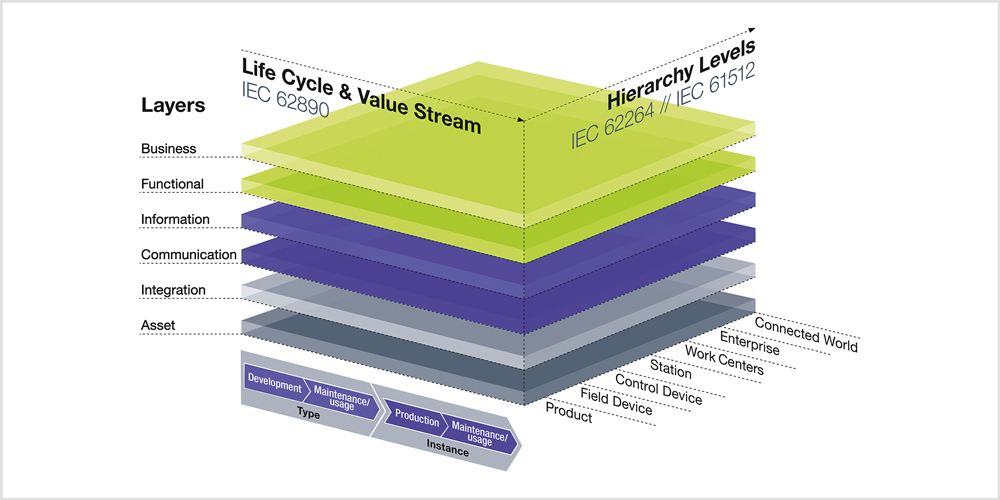
\includegraphics[width=0.95\textwidth]{img/rami40-ebenenmodell.png}
            \caption{RAMI 4.0 as a layered model \cite{rami_img_source}}
            \label{figure:rami-layers}
        \end{figure}

        \noindent The left horizontal axis ``Lifecycle \& Value Stream'' shows the lifecycle of products in the IIoT system, especially with regard to data collection, and follows the IEC 62890 standard. The lifecycle is grouped into two sections, starting the ``Type''. This section represents prod\-ucts that are prototypes and still in development which is why it is further subcategorized into the parts ``Development'' which deals with actual development and construction of the production and ``Maintenance/Usage'' which concerns with software updates, manuals or product changes. The second section called ``Instance'' deals with products that are finished already. It also has two subcategories, in particular ``Production'' which deals with production-relevant data like quality measurements, serial numbers, etc. and ``Maintenance/Usage'', again focusing on operational tasks like maintenance, optimizations, updates and more.\newline

        \noindent Lastly, the right horizontal axis is named ``Hierarchy Levels'' and follows the IEC 62264 / IEC 61512 standards which include an international norm for the integration of enterprise IT and control systems. The IEC 62264 standard also includes the automation pyramid discussed in \autoref{subsection:automation-pyramid} which is why strong similarities to the automation pyramid can be found in the legend of this axis. Apart from the new parts ``Product'', which focuses on the actual product under observation rather than sensors or actuators interacting with it, and ``Connected World'' which allows to portray today's internet-based approach to connecting production facilities over the network. Overall this layer shows the different functionalities within a production facility/ecosystem.

        As mentioned earlier, the RAMI 4.0 model provides a basis for discussion. For instance, this allows to place other standards or norms into the three-dimensional model. This can help to detect overlaps or even gaps when evaluating or discussing frameworks or technologies. In summary, the model fits the use case of discussing, planning and designing IIoT systems perfectly, but is not aimed towards actual implementation and is hence not well suited for the purposes of the implementation-focused and practical goals of this thesis \cite{koschnick_industrie_nodate}.

    \subsubsection*{The Industrial Internet Reference Architecture (IIRA)}
    \label{subsubsection:iira}
        Another common standard in the field of reference architectures for IIoT is the ``Industrial Internet Reference Architecture'' (IIRA). The IIRA aims to address the need for a common architecture framework to develop interoperable IIoT systems for diverse applications across a broad spectrum of industrial verticals in the public and private sectors to achieve the true promise of IIoT, with focus on broad applicability, interoperability and identification and satisfaction of stakeholder needs. It was created by the ``Industry IoT Consortium'' and is based on the ISO/IEC/IEEE 42010:2011 standard \cite{iiot_consort_iira}. Seen from a high-level perspective, the IIRA highlights the important architectural concerns of IIoT systems and classifies them into so-called ``viewpoints'' along with their respective stakeholders like product managers, developers or system operators. Based on this classification the IIRA proceeds to provide guidance to resolve the concerns in these viewpoints.

        \begin{figure}[htbp]
            \centering
            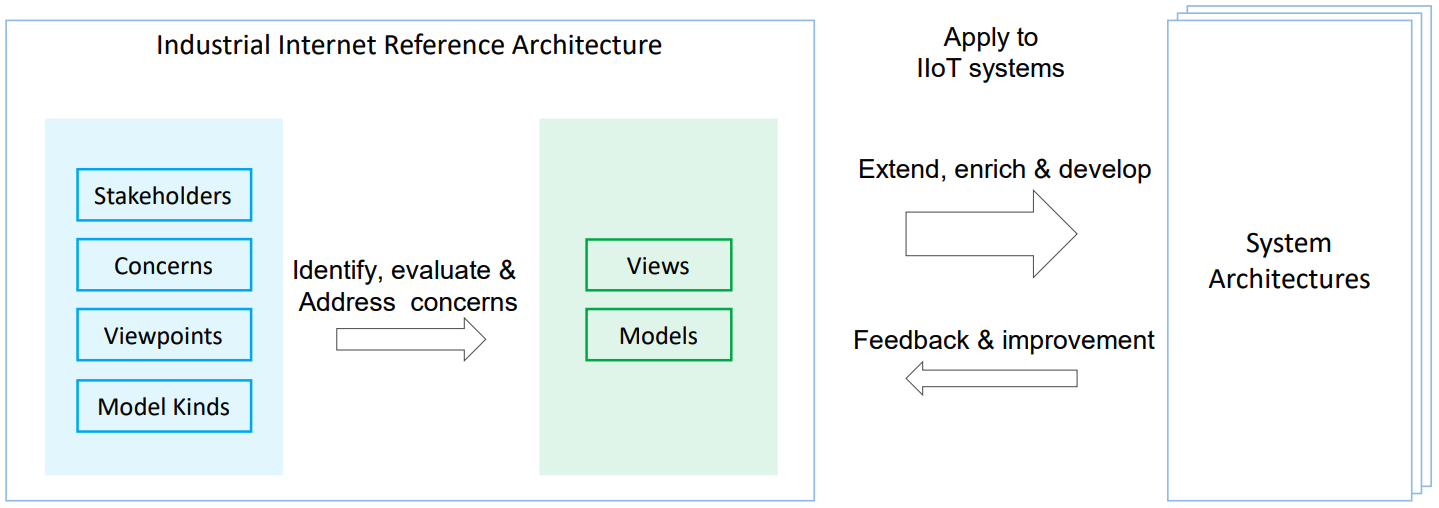
\includegraphics[width=0.9\textwidth]{img/iira.png}
            \caption{IIRA Constructs and Application \cite{koschnick_industrie_nodate}}
            \label{figure:iira-process}
        \end{figure}

        \newpage

        \autoref{figure:iira-process} shows the workflow of using the IIRA. In the first step, stakeholders and their concerns are identified. Based on these identified concerns, the architect maps the stakeholder concerns into a set of predefined viewpoints. These viewpoints are the business viewpoint, which focuses on business-related aspects of the system, the usage viewpoint, which looks at how users will interact with the system, the functional viewpoint, which concerns with the system's functional requirements and capabilities and finally the implementation viewpoint that revolves around the technical realization of the system. Note that in the IIRA, the viewpoints are arranged in an order that reflects the general interaction pattern between them. Decisions from a higher-level viewpoint (e.g. business viewpoint) guide and impose requirements on the viewpoints below it while lower viewpoints validate and in some cases cause revisions to the analysis and decisions in the viewpoint above it. Some crosscutting concerns might also intersect multiple or even all viewpoints, such as safety and security. As the last component of the left section in the figure, the IIRA provides a set of predefined model kinds that are the types or categories of models that are relevant to the viewpoints. A model kind can also be described as a blueprint for a model that specifies syntax, semantics, rules and more. 
        Based on all of these parts, specific ``views'' and ``models'' are developed for each viewpoint. Views are representations of the system from the perspective of a specific viewpoint hence they are also specific to one or more stakeholders. An example is a view for a security viewpoint, which would for example include security concerns like authentication, authorization and confidentiality. Models on the other hand are detailed representations within the views. They are developed based on the defined model kinds for the according viewpoint and are typically structural, behavioral or domain-specific. Following the security viewpoint example, a model might show, how a user's identity is verified in the IIoT system. As with any kind of reference architecture, the model is then used to extend, enrich and develop the real system architecture. From learnings during development, the model based on the IIRA can be adapted through the feedback \& improvement step, thus resulting in a continuous cycle of refinement \cite{iiot_consort_iira}. \newline 

        While the process described so far mostly deals with requirements engineering, the IIRA also recommends well-established architecture patterns for IIoT including a three-tier architecture, pub-sub architectures or layered data bus that verify concepts mentioned in this thesis, especially in \autoref{chapter:architecture-proposal}. 
        The three-tier architecture pattern comprises edge, platform and enterprise tiers and suggests dividing the system into three ``tiers'', where each tier has its own responsibilities. This for example allows for practices like edge computing mentioned in \autoref{section:edge-computing} and cloud computing. The pub-sub architecture is the basis for the communication protocol MQTT which was discussed in \autoref{subsubsection:mqtt} and is also mentioned as an example concrete technology for the message/data broker functionality in the IIoT system. Lastly, the layered data bus pattern suggests having multiple data buses, which might be a message broker like an MQTT broker, on different levels, where levels might, for example, be instances of the tiers of a three-tier architecture. It allows to have local communication compared to a centralized, often cloud-based, data bus, where all communication has to go to a central location first. Communication between layers only happens between data buses, so no direct communication channels are used which helps with decoupling system components. By applying the layered data bus pattern, requirements like low latency, peer-to-peer communication, ability to work offline (important for manufacturing) or secure network segregation can be fulfilled. All of the just mentioned patterns will also be applied in the architecture proposal of this thesis in \autoref{chapter:architecture-proposal}, which confirms that the suggested architecture proposal is well-aligned with established practices and principles in the field. Note that the IIRA mentions more patterns or capabilities relevant to IIoT systems like time-series databases or stream analytics which go beyond the scope of this work.
        
        In summary, the IIRA outlines key concepts pertinent to IIoT systems, offering wide-ranging applicability across various industrial sectors. Its focus is primarily on the overarching system architecture and the generic aspects of IIoT systems. This contrasts with RAMI 4.0 detailed in \autoref{subsubsection:rami-40}, which is specifically tailored to smart manufacturing and the core principles of Industry 4.0 and less towards system architecture. The IIRA mentions patterns that are similarly structured to modern IIoT architectures and speaks about their benefits. In contrast to older architectures like the automation pyramid discussed in \autoref{subsection:automation-pyramid} it also supports requirements for modern IIoT systems like scalability or even concepts like edge computing. The IIRA is however at a level of abstraction, that excludes architectural elements that are only available in concrete systems and is not at a depth sufficient to implement a real system. The reference architecture is best used for planning and designing a large-scale IIoT system whereas other guidance should be used for the actual implementation of the system \cite{iiot_consort_iira}.
        